\section{Ejercicio 6}

En este ejercicio la idea es entrenar una red neuronal para que aprenda la regla XOR que tiene dos entradas (1 y -1) y sigue la regla: "Si las entradas son iguales la salida es -1 y si son distintas entonces la salida es 1". Para ello se propone utilizar los conceptos de programación orientada a objetos y dos arquitecturas como las que se muestran a continuación:

\begin{figure}[H]
    \centering
    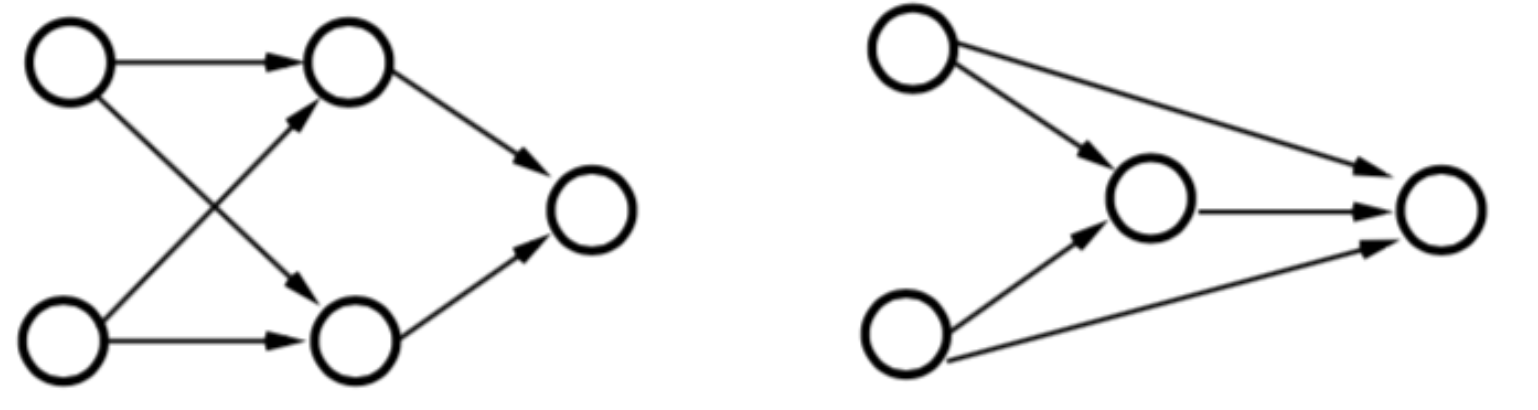
\includegraphics[width=0.5\textwidth]{image/archs.png}
    \caption{Arquitecturas propuestas para resolver el problema de aprendizaje de la regla XOR.}
    \label{fig:archs}
\end{figure}

Ambas arquitecturas cuentan con una capa de entrada de datos, una capa oculta y una capa de salida. La diferencia subyace en que en la primera arquitectura todos la salida se obtiene directamente de los resultados de la capa intermedia u oculta, mientras que en la segunda arquitectura se propone que los datos de salida se obtengan utilizando tanto de los resultados de la capa intermedia como los datos de entrada.

Cada capa tiene como función de activación la función \textbf{tangente hiperbólica} y se utiliza la función MSE como función de Costo. 
Para resolver el problema se propone una estructura de código que no se explicará en este informe pero que puede consultarse en \cite{tomas2}.

Una vez implementado el código que resuleve el problema, se utilizan los métodos \textbf{add} de la clase \textit{Models} y \textbf{Dense} y \textbf{Concatenate} ambos de la clase \textit{layers} para generar cada arquitectura. Notar que solo se trabajarán con capas densas en este trabajo.

\begin{figure}[H]
    \centering
    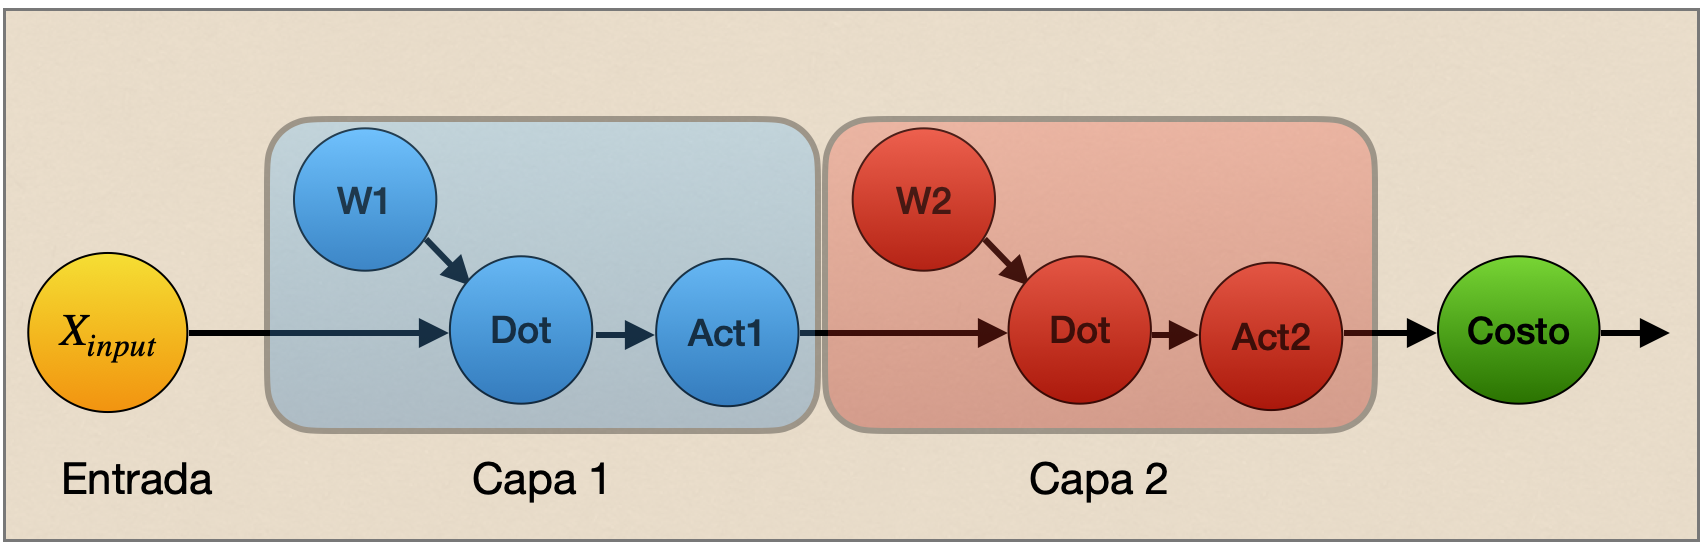
\includegraphics[height=1.5in]{image/graph_8_a.png}
    \caption{Grafo computacional de la primera arquitectura}
    \label{fig:graph6a}
\end{figure}

Entonces, para crear la primera arquitectura se arma el grafo computacional de la Fig.~\ref{fig:graph6a} se realiza el siguiente algoritmo:

\begin{verbatim}
    # Dataset: se crean los datos de entrada
    x_train = np.array([[-1, -1], [-1, 1], [1, -1], [1, 1]])
    y_train = np.array([[1], [-1], [-1], [1]])

    # Create model: 1st architecture
    model = models.Network() # se crea la red vacía
    model.add(layers.Dense(units=2, activation=activations.Tanh(),
        input_dim=x_train.shape[1]))  # agregamos la primera capa
    model.add(layers.Dense(units=1, activation=activations.Tanh()))# agregamos la segunda capa

    # Train Network: entrenamiento de la red
    model.fit(x_train, y_train, test_data=None, epochs=3000, loss=losses.MSE(),
        opt=optimizers.BGD(lr=0.01, bs=x_train.shape[0]), name=problem_name)  
\end{verbatim}


Con esta arquitectura y con los parámetros mencionados los resultados obtenidos para el Accuracy y la Loss son los siguientes:

\begin{figure}[H]
     \centering
     \begin{subfigure}[b]{0.45\textwidth}
         \centering
         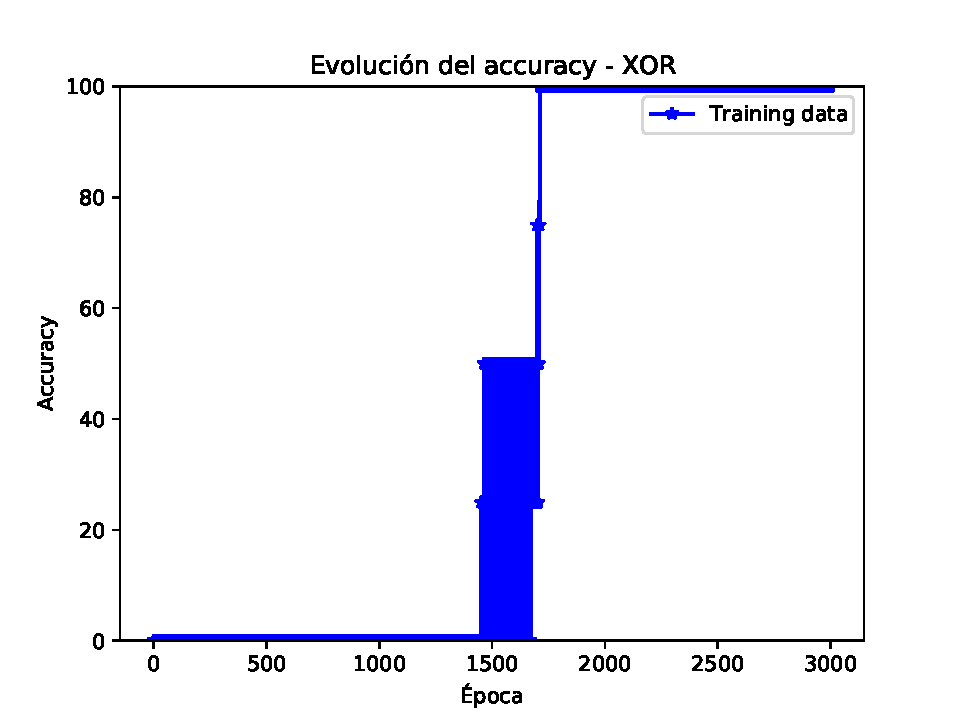
\includegraphics[width=\textwidth]{image/TP2_6_acc_a.pdf}
         \caption{Accuracy para el problema de aprendizaje de la regla XOR para la primera arquitectura presentada}
         \label{fig:acc6a}
     \end{subfigure}
     \hfill
     \begin{subfigure}[b]{0.45\textwidth}
         \centering
         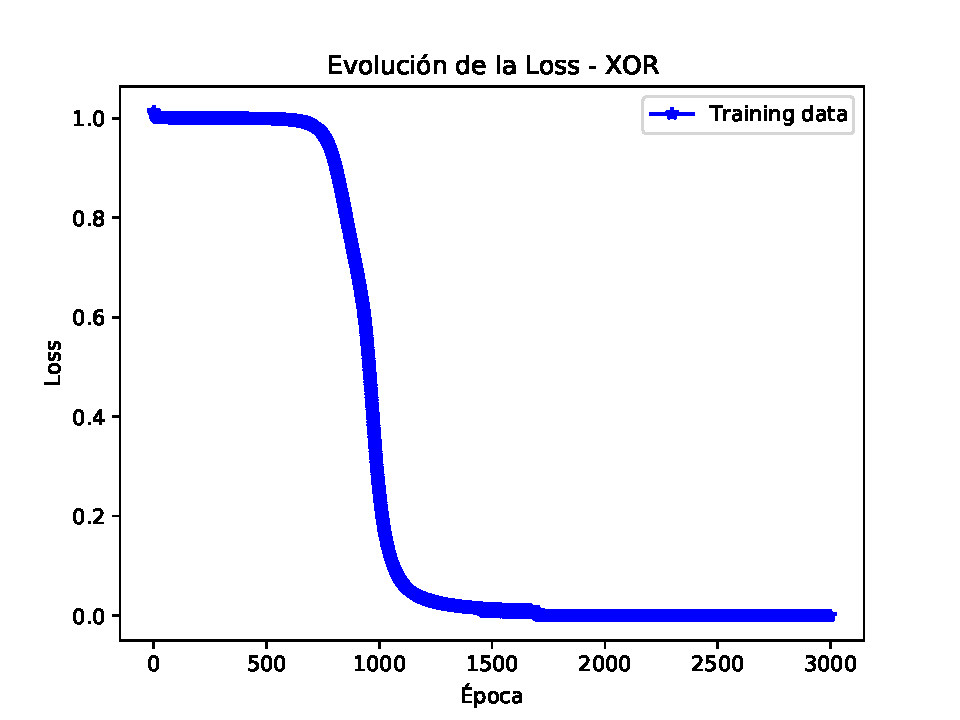
\includegraphics[width=\textwidth]{image/TP2_6_Loss_a.pdf}
         \caption{Loss para el problema de aprendizaje de la regla XOR para la primera arquitectura presentada}
         \label{fig:loss6a}
     \end{subfigure}
        \caption{Resultados para la primera arquitectura presentada para resolver el problema de la regla XOR con dos capas densas}
        \label{fig:resu6a}
\end{figure}

Para implementar la segunda arquitectura se utilizaron las siguientes líneas de código:

\begin{verbatim}
    # Create model: 2nd architecture
model = models.Network()
# se crea la primera capa densa
model.add(layers.Dense(units=2, activation=activations.Tanh(),input_dim=x_train.shape[1])) 
# se concatena la salida de la capa creada con los datos de entrada
model.add(layers.Concatenate(x_train.shape[1]))
# se crea la capa densa de salida
model.add(layers.Dense(units=1, activation=activations.Tanh()))
# Train Network
model.fit(x_train, y_train, test_data=None, epochs=3000, loss=losses.MSE(), 
    opt=optimizers.BGD(lr=1e-2, bs=x_train.shape[0]), name=problem_name, reg=None)
    #regularizers.L2(lam=1e-6))
\end{verbatim}
donde \textit{Concatenate} genera una pesudo capa oculta que permite concatenar la salida de la primera capa oculta con la entrada del sistema. El grafo computacional por el que se puede respresentar esta arquitectura se muestra en la Fig.~\ref{fig:graph8b}.

\begin{figure}
    \centering
    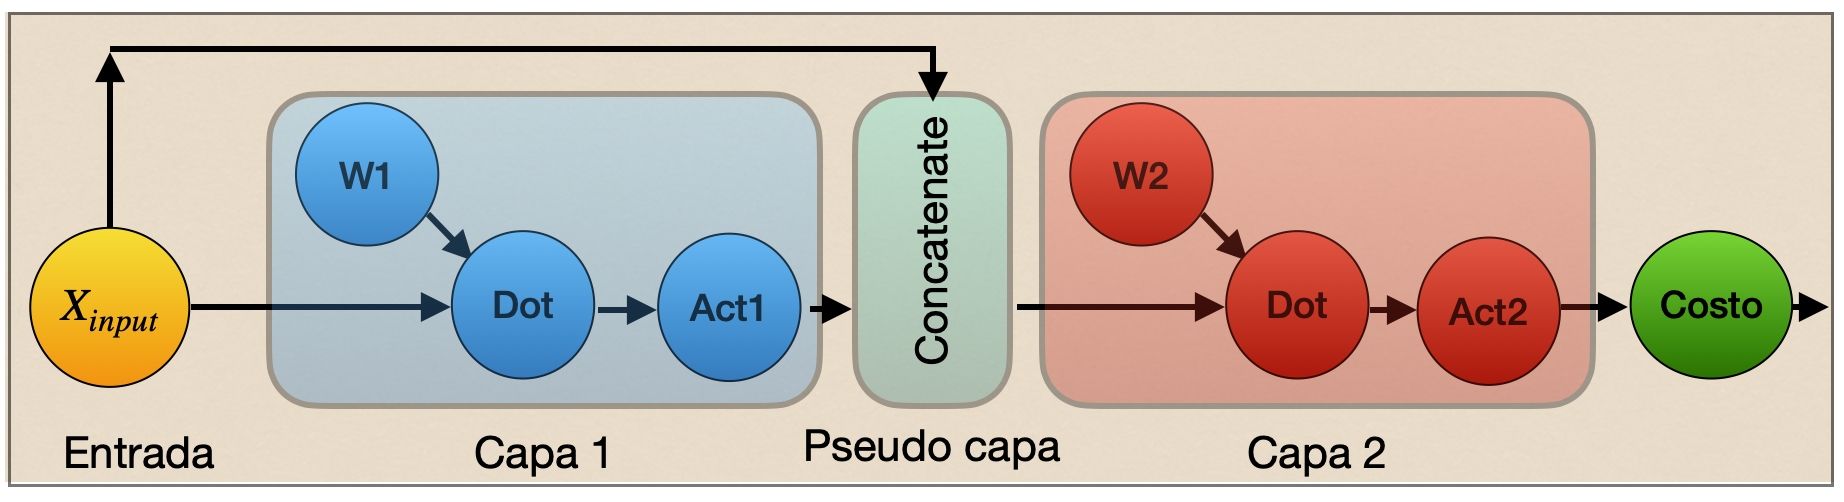
\includegraphics[height=1.5in]{image/graph_8_b.png}
    \caption{Grafo computacional de la segunda arquitectura}
    \label{fig:graph8b}
\end{figure}

Los resultados del accuracy y la loss para esta segunda arquitectura resultó:

\begin{figure}[H]
     \centering
     \begin{subfigure}[b]{0.45\textwidth}
         \centering
         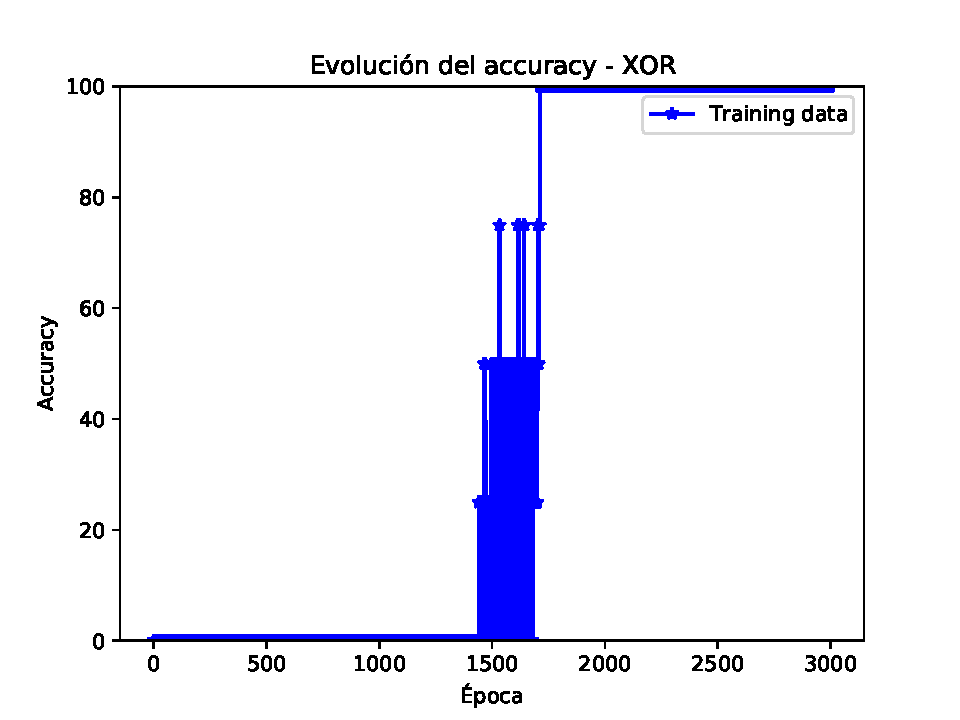
\includegraphics[width=\textwidth]{image/TP2_6_acc_b.pdf}
         \caption{Accuracy para el problema de aprendizaje de la regla XOR para la segunda arquitectura presentada}
         \label{fig:acc6a}
     \end{subfigure}
     \hfill
     \begin{subfigure}[b]{0.45\textwidth}
         \centering
         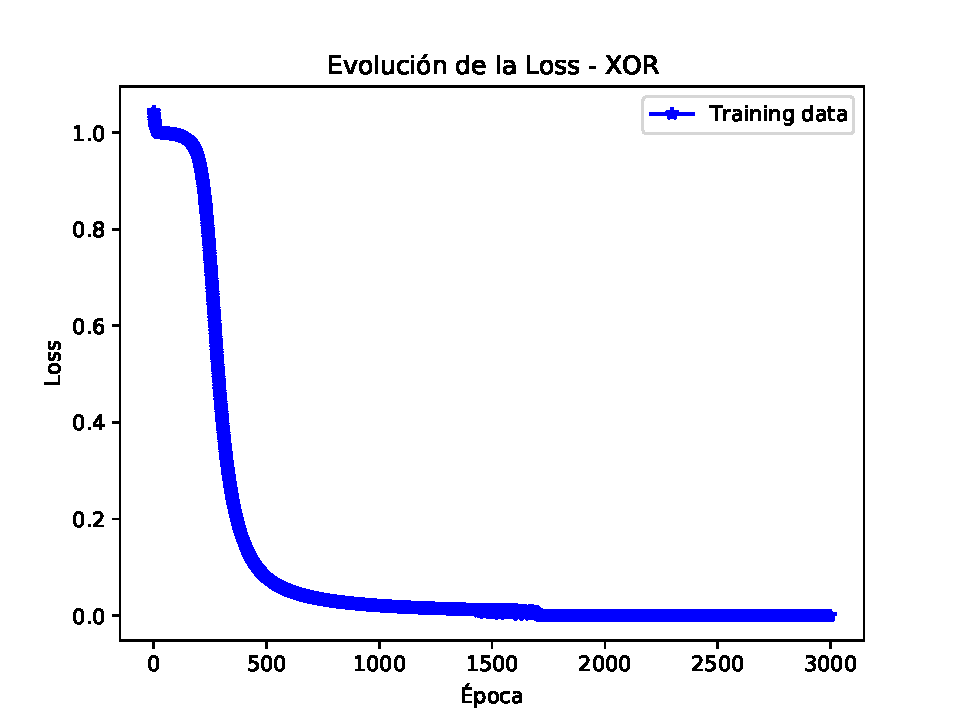
\includegraphics[width=\textwidth]{image/TP2_6_Loss_b.pdf}
         \caption{Loss para el problema de aprendizaje de la regla XOR para la segunda arquitectura presentada}
         \label{fig:loss6a}
     \end{subfigure}
        \caption{Resultados para la segunda arquitectura presentada para resolver el problema de la regla XOR con dos capas densas}
        \label{fig:resu6a}
\end{figure}

